\documentclass[12pt]{article}

\usepackage{graphicx}
\usepackage{enumerate}
\usepackage{listings}
\usepackage{multicol}

\lstMakeShortInline|
%\linespread{1.6}

\title{Live Map of the DC Bus System (Bus Tracker): Design}
\author{Ian Will, Jason Cluck}
\date{}

\begin{document}
\maketitle

\section*{Introduction}
	Public transportation in the District of Columbia is very important to most of it's residents and employees.  This project aims to provide users with recent bus data to ensure the most productive transportation.  The project will manifest as a web application named Bus Tracker that can be accessed through any device capable of supporting a web browser.  Some of the useful data that will be provided through this application will be the buses' current location, their expected arrival times, and current headsign.  This information provides more information to transit riders than previous tools, which only provide expected arrival times of a bus at a specific stop.

\section*{Design}

The project to create a live map of DC's Washington Metro Area Transit Authority (WMATA) bus system will be built using the Ruby on Rails web framework, the Google Maps API, WMATA's Transparent Data Sets API, and Twitter's Bootstrap CSS API.

The Google Maps API is used to display the background map, route paths, and bus marker overlays.  Figure \ref{fig:designOverview} shows an overview for how these APIs connect to the Rails web server we're building.

\begin{figure}[ht]
	\centerline{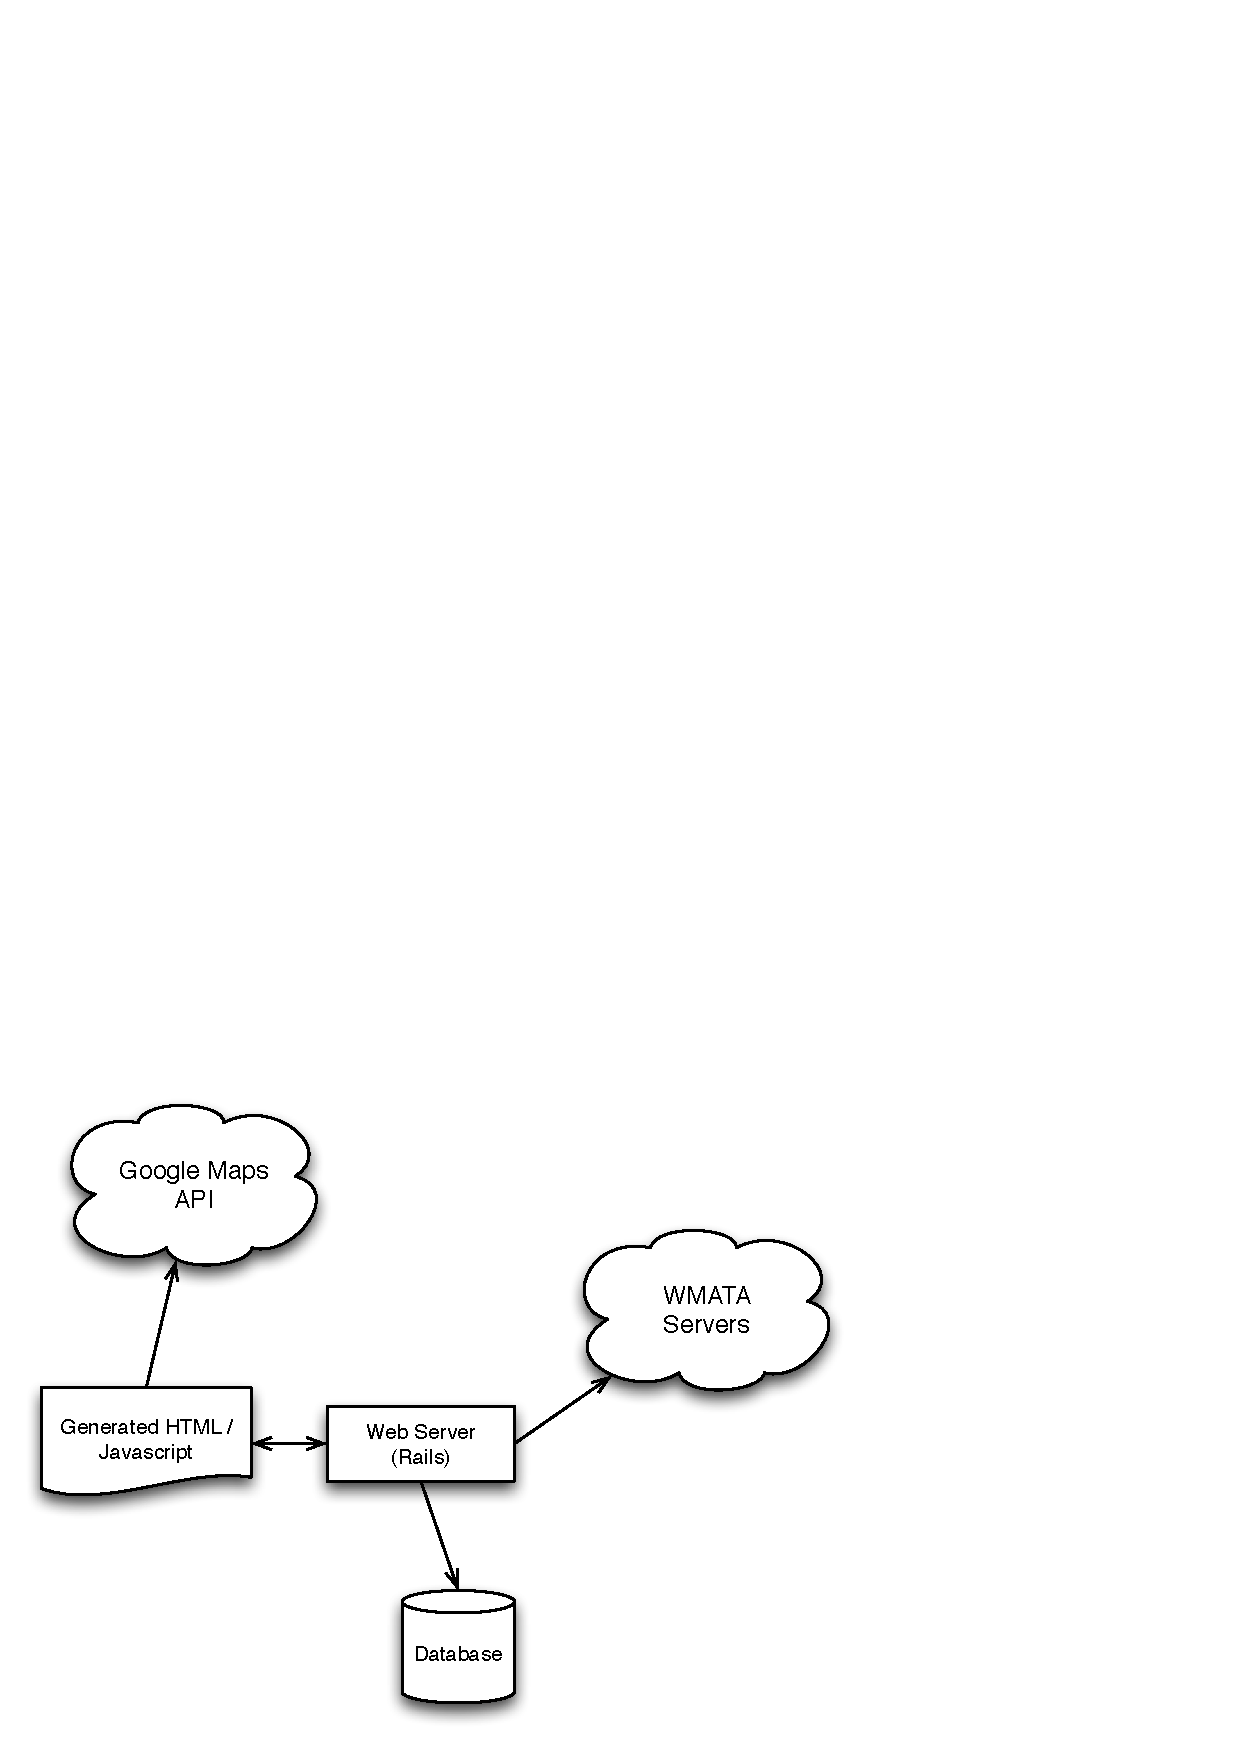
\includegraphics[scale=0.6]{design.png}}
	\caption{API integration overview}
	\label{fig:designOverview}
\end{figure}

The Rails design philosophy favors adopting standard conventions for naming, folder structure, and design patterns across all Rails applications.   This accelerates web development, saving a lot of configuration and rudimentary structuring and naming decision when starting a project.  It also allows the framework to provide numerous helper tools that automate as much as possible.


\subsection*{Model-View-Controller}
The fundamental design pattern adopted by Rails is Model-View-Controller (MVC).  The premise behind MVC is to separate user-interface code (the View), data structures (the Model), and the business logic that connects them (the Controller) into separate modules that can be developed, unit tested, and maintained in isolation.  Figure \ref{fig:MVC} shows the MVC separation as used in the Bus Tracker application.

\begin{figure}[ht]
	\centerline{\includegraphics[scale=0.55]{busTrackerUML.png}}
	\caption{MVC control pattern}
	\label{fig:MVC}
\end{figure}

When an HTTP request comes to the HTTP Server, it first goes to the rails router, which determines which Controller should handle that request.  The controller then uses the Model classes to get the current state of data (e.g. the current position of buses from the database), and passes that information to the View classes.  Rails stores the View logic as HTML with additional preprocessor directives for special scripts called ``partials'' including Embedded Ruby and CoffeeScript.  When these partials are processed by the appropriate preprocessor engine, they have access to variables and data structures provided by the controller.  The preprocessor engine dynamically generates standard HTML and Javascript based on the partial scripts and the data provided by the controller.  These conventions and tools make it easy to prevent business logic from creeping into view code.  They provide a standard idiom for passing data between the model, controller, and view.

Rails adopts the Representational State Transfer (REST) architecture for the HTTP interface.  It uses the inherent HTTP methods (GET, POST, PUT, DELETE) to execute the corresponding Create, Read, Update, Destroy (CRUD) operations on the data model.  This approach is contrasted by the alternative (non-REST) approach of relying predominantly on the HTTP GET method and controlling CRUD behavior using special parameters embedded in the URI.  Our Bus Tracker application doesn't provide a user-facing capability to create, update, or destroy the model since model updates are fetched from WMATA servers rather than driven by user input.  Therefore the POST, PUT, and DELETE routes have no action associated with them in the controller.  

The GET requests retrieve different types of data depending on the URI requested.  Requesting the root (GET / or GET /index.html) provides the overview map display.  Requesting \lstinline|GET /buses| or GET /buses.json returns the current state of the buses model.  Request GET /stops requests data purely on the stops.  These likely won't be used directly by users, but they are used in the Javascript that asynchronously updates the map display.  Periodically a Javascript request is made to /buses.json to retrieve an updated array of bus positions in the JSON format.  

Some of the API features specific to Bus Tracker are listed in Figure \ref{fig:MVC}.  The controller relies on fetching data from the WMATA servers which  are accessed via a helper class - WmataHelper.  WmataHelper fetches the current position of all buses from the WMATA servers and stores that data in using the model classes. 

 Bus Tracker also uses is Twitter's Bootstrap API which provides additional CSS options. Combining Bootstrap with the View can create dynamic web pages that can render correctly on phones or desktop computers with minimal overhead.

\subsection*{Model Relationships}

Bus Tracker will contain information regarding all the buses served by WMATA.  This includes bus information (including positions), stop information, and route information (including way points describing the route).  Figure \ref{fig:busEntity} shows the entities and relationships between the WMATA data used by Bus Tracker.  This is the information that will be stored locally after retrieving the information from WMATA.

\begin{figure}[ht]
	\centerline{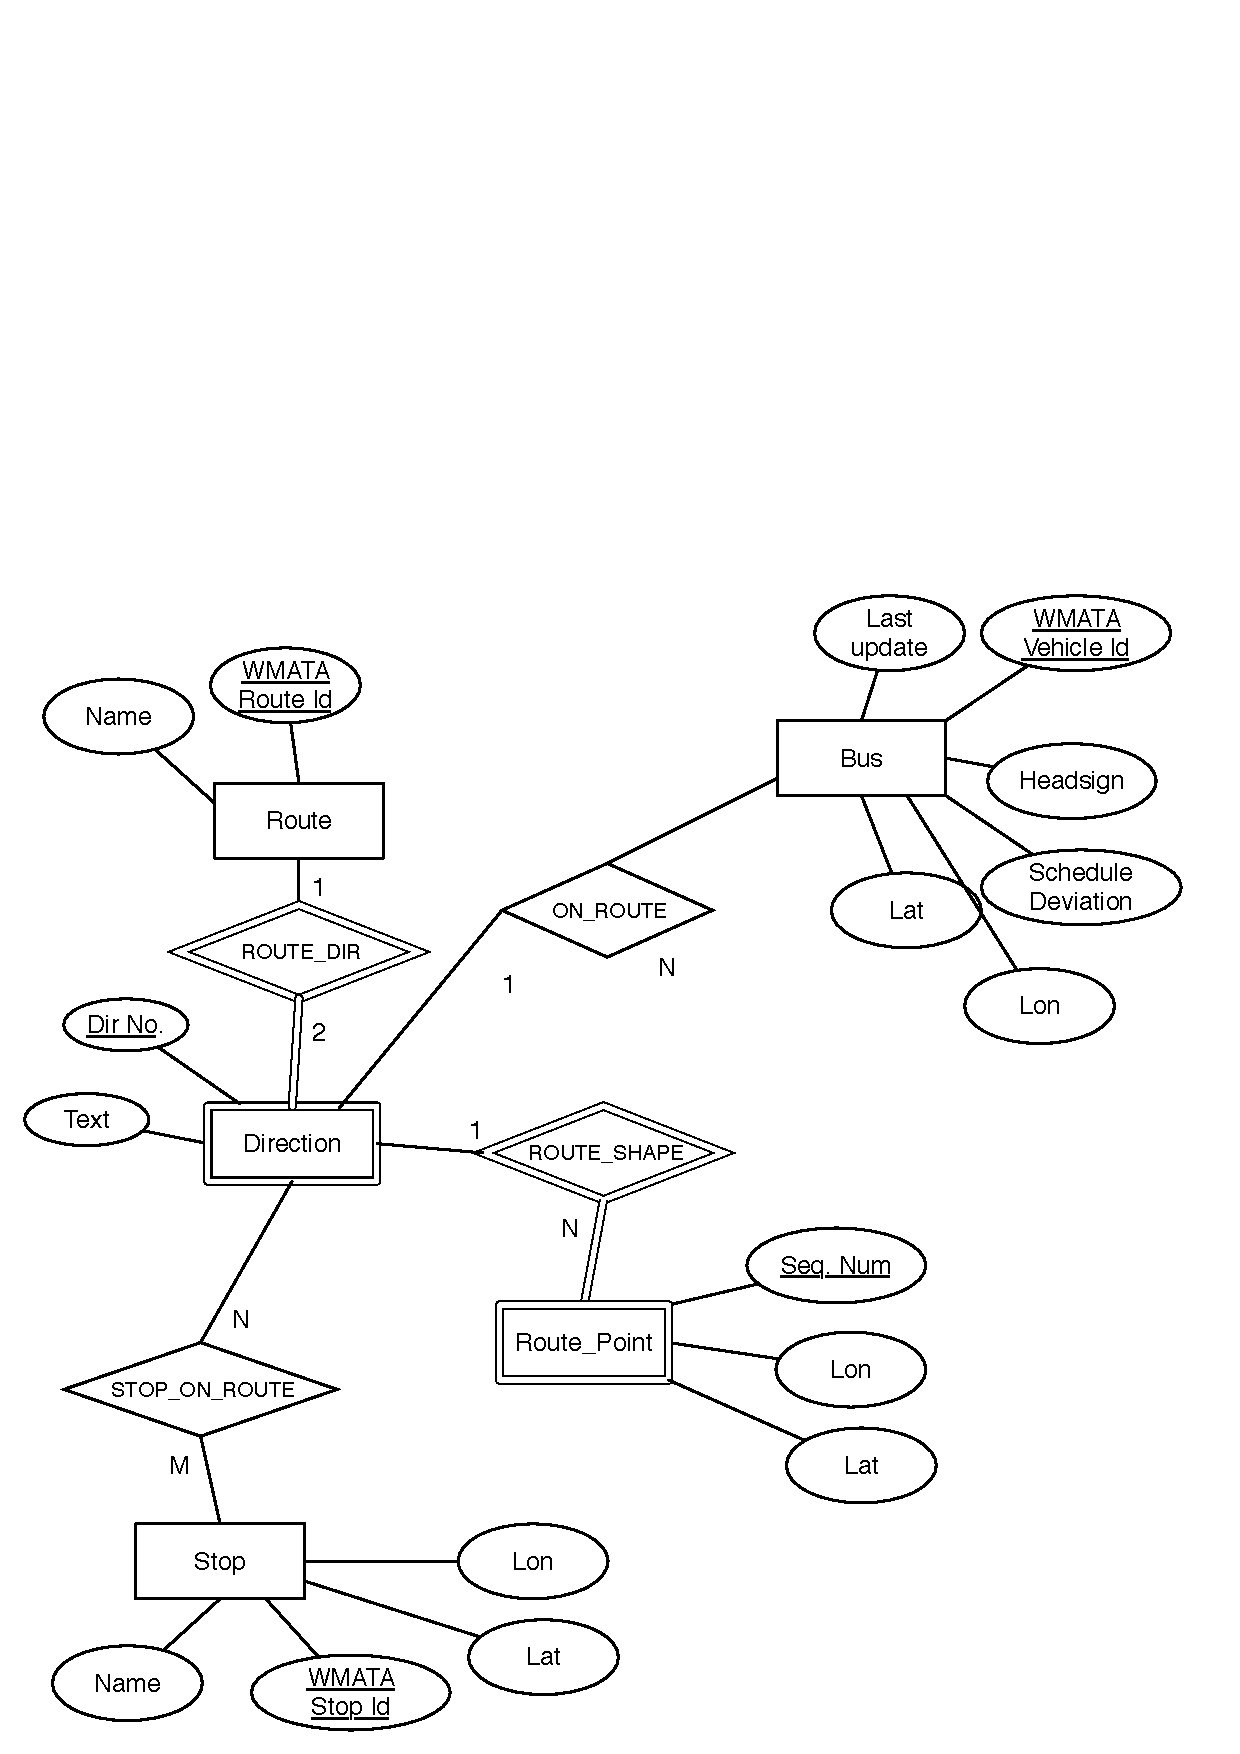
\includegraphics[scale=0.43]{bus-entity-rel.png}}
	\caption{Model relationship diagram}
	\label{fig:busEntity}
\end{figure}

Figure \ref{fig:busSchema} shows the schema that Bus Tracker uses to store information about the current state of the WMATA bus system.  This persists all necessary information on routes, buses, and stops.  Underlined fields indicate primary keys, arrows indicate foreign key dependencies on primary keys from other tables.  

\begin{figure}[ht]
	\centerline{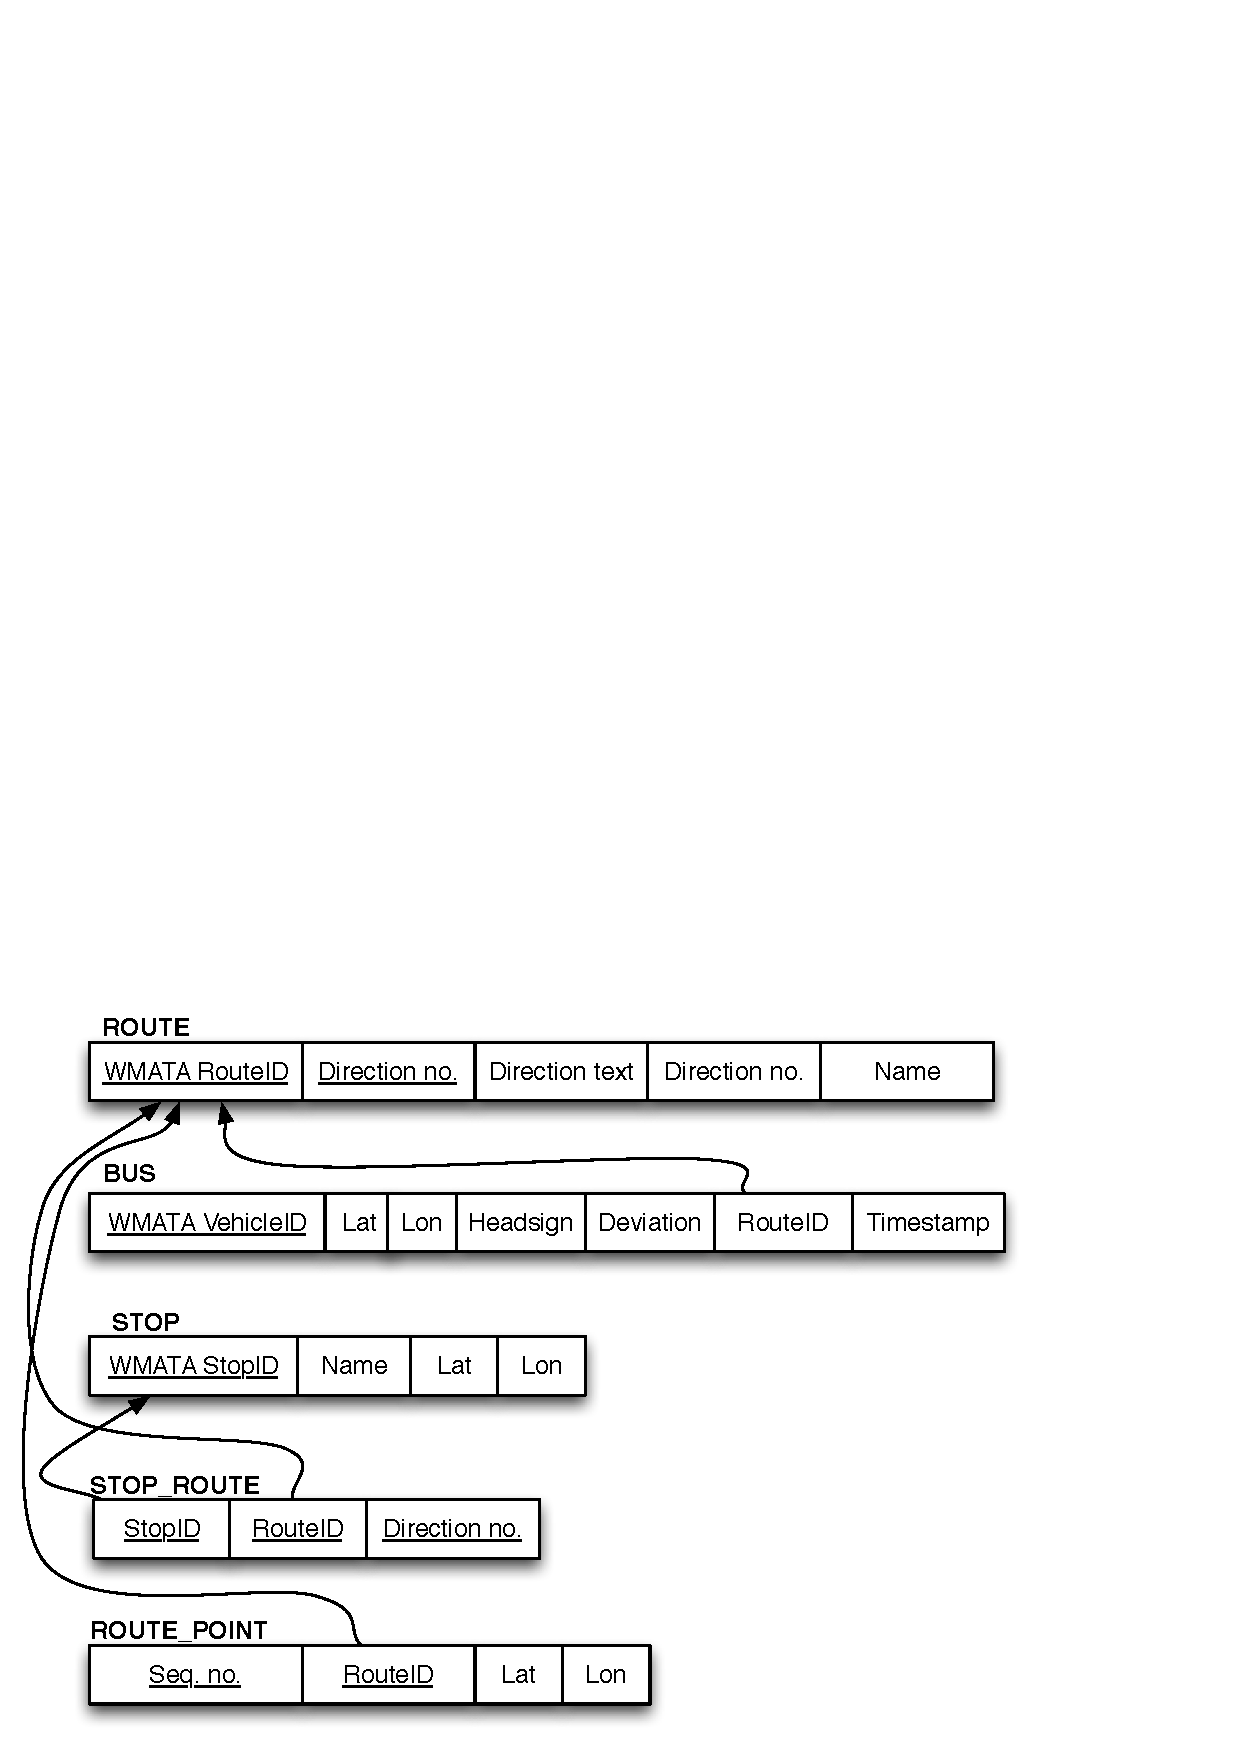
\includegraphics[scale=0.6]{bus-schema.png}}
	\caption{Schema for WMATA API}
	\label{fig:busSchema}
\end{figure}


\section*{Task Breakdown and Timeline}
\begin{description}
	\item Tasks to be done by:  November 10, 2012  	
	
	\begin{enumerate}
		\item Initial rails setup [Cluck]
		\item CSS styling using twitter bootstrap [Cluck]
		\item Display map on index page [Cluck]
		\item Fetch bus positions from WMATA servers [Will]
		\item Store WMATA response in database [Will]
		\item Draw markers on map for bus locations [Will]
		\item Draw lines on map for bus routes [Will]
		\item Display initial map area based on geo-location reading [Cluck]
		\item Show info window when bus marker is clicked, including the following [Will]
		\begin{enumerate}
			\item Route name
			\item Schedule deviation (lateness)
			\item Time of last position update (data staleness)
			\item Headsign
			\item Direction
		\end{enumerate}
	\end{enumerate}
	\item Tasks to be done by: November 20, 2012
	\begin{enumerate}
		\item Fetch routes from WMATA servers [Will]
		\item Fetch stops from WMATA servers [Will]
		\item Store routes in database [Cluck]
		\item Store stops in database [Cluck]
		\item Layer toggle widget that shows Google traffic overlay, bus markers, and stop markers [Will]
	\end{enumerate}
	\item Tasks to be done by: December 3, 2012
	\begin{enumerate}
		\item Display bus stops with markers on map [Cluck]
		\item Control WMATA polling to avoid exceeding usage limits [Will]
		\item Show info window when stop marker is clicked [Will]
			\begin{enumerate}
				\item Show which routes and directions the use the stop
				\item Show next bus wait time projections for each route that uses the stop
			\end{enumerate}
		\item Add iOS/Android functionality using mobile web browser [Cluck]
	\end{enumerate}
\end{description}
\end{document}

